% !TEX program = xelatex

\documentclass[titlepage]{article}

\usepackage{geometry}

\usepackage{polyglossia}
\setdefaultlanguage{greek}
\setotherlanguage{english}

\usepackage{fontspec}
\setmainfont{Noto Serif}
\setsansfont{Noto Sans}
\setmonofont{Noto Mono}
\newfontfamily\greekfont{Noto Serif}
\newfontfamily\greekfontsf{Noto Sans}
\newfontfamily\greekfonttt{Noto Mono}

\usepackage{graphicx}
\graphicspath{{../plots/}}
\usepackage{subcaption}

\usepackage{booktabs}

\usepackage[hidelinks]{hyperref}

\begin{document}

\title{Κατανεμημένα Συστήματα\\
    Εξαμηνιαία Εργασία\\
    Noobcash}
\author{Αλέξιος Ζαμάνης\\
    03115010\\
    Ελένη Στραϊτούρη\\
    03115068}

\maketitle

\tableofcontents

\section{Εισαγωγή}

Στα πλαίσια της εργασίας μελετήσαμε το blockchain και τις εφαρμογές του στα ψηφιακά νομίσματα. Συγκεκριμένα χρησιμοποιήσαμε το blockchain για να υλοποιήσουμε ένα κρυπτονόμισμα στα πρότυπα του Bitcoin ονόματι Noobcash. Στη συνέχεια εκτελέσαμε μια σειρά από πειράματα και αξιολογήσαμε το σύστημά μας ως προς την απόδοση και την κλιμακωσιμότητά του βάσει δύο μετρικών και για διάφορες τιμές των παραμέτρων του. Παρακάτω περιγράφουμε την αρχιτεκτονική του συστήματός μας. Στη συνέχεια παραθέτουμε τα αποτελέσματα των πειράματών μας συνοδευόμενα από σύντομο σχολιασμό.

\section{Ζητήματα των ψηφιακών νομισμάτων}

Το Noobcash είναι ένα ψηφιακό νόμισμα. Επομένως η κύρια λειτουργία που καλείται να επιτελέσει το σύστημά μας είναι η διεκπεραίωση συναλλαγών μεταξύ των χρηστών. Μια συναλλαγή συνίσταται στην ουσία στη μεταφορά Noobcash από ένα χρήστη σε έναν άλλο. Προφανώς, δεδομένης της φύσης των ψηφιακών νομισμάτων, προκύπτει ένα σύνολο ζητημάτων κατά την επαλήθευση της ορθότητας των συναλλαγών, τα οποία το σύστημά μας οφείλει να επιλύσει. Ακολούθως παραθέτουμε τα σημαντικότερα εξ αυτών μαζί με τη λύση την οποία υιοθετεί το Noobcash.

\subsection{Authentication και integrity}

Έστω ότι μια συναλλαγή είναι μια εγγραφή αποτελούμενη από ένα αποστολέα, ένα παραλήπτη και ένα ποσό από Noobcash. Οφείλουμε να επιβεβαιώσουμε ότι ο αναγραφόμενος αποστολέας πράγματι δημιούργησε τη συναλλαγή και ότι ο παραλήπτης και το ποσό που αναγράφονται είναι πράγματι αυτά που επιθυμεί ο αποστολέας. Το πρώτο πρόβλημα συνίσταται στην ουσία στην επαλήθευση της ταυτότητας του αποστολέα, ενώ το δεύτερο στην επαλήθευση της ακεραιότητας των δεδομένων. Αμφότερα τα προβλήματα λύνονται με τη χρήση ψηφιακών υπογραφών.

\paragraph{Ασύμμετρη κρυπτογράφηση}

Για τη χρήση ψηφιακών υπογραφών κάθε αποστολέας δημιουργεί ένα ζεύγος κλειδιών χρήσει των τεχνικών της ασύμμετρης κρυπτογράφησης. Το ένα κλειδί είναι ιδιωτικό και ως εκ τούτου γνωστό μόνο στον αποστολέα. Το άλλο κλειδί είναι δημόσιο και πρέπει να είναι ελεύθερα διαθέσιμο σε όποιον επιθυμεί να επαληθεύσει τη συναλλαγή. Ό,τι κρυπτογραφείται με το ιδιωτικό κλειδί μπορεί να αποκρυπτογραφηθεί μόνο με το δημόσιο και το αντίστροφο. Επομένως αν αποκρυπτογραφήσουμε επιτυχώς ένα μήνυμα, γνωρίζουμε ότι κρυπτογραφήθηκε από τον αποστολέα (επαλήθευση ταυτότητας) και ότι δεν έχει αλλοιωθεί κατά τη μεταφορά (ακεραιότητα δεδομένων), καθώς ο επιτιθέμενος δε θα μπορούσε επιτυχώς να κρυπτογραφήσει την αλλοιωμένη εκδοχή.

\paragraph{Ψηφιακές υπογραφές}

Η κρυπτογράφηση είναι αρκετά δυνατή, ώστε πλέον των παραπάνω να μας προσφέρει και εμπιστευτικότητα, που ωστόσο δε μας ενδιαφέρει, ενώ μάλιστα κοστίζει σε υπολογιστικό χρόνο, καθώς η κρυπτογράφηση είναι υπολογιστικά βαριά. Ως εκ τούτου δεν κρυπτογραφούμε την ίδια τη συναλλαγή, αλλά το hash της. Το hash αποτελεί μια μικρή, σταθερού μήκους συμβολοσειρά, που αντιπροσωπεύει μοναδικά με πολύ μεγάλη πιθανότητα το μήνυμά μας, χωρίς βέβαια κάποιος που γνωρίζει το hash να μπορεί να εκμαιεύσει το αρχικό μήνυμα. Επομένως αν αλλάξει το μήνυμα, θα πρέπει να αλλάξει και το hash για να αντιστοιχεί στο νέο μήνυμα, πράγμα αδύνατο, καθώς το hash είναι κρυπτογραφημένο. Αυτό το κρυπτογραφημένο hash καλείται ψηφιακή υπογραφή.

\paragraph{}

Συμπεραίνουμε επομένως πως κάθε επίδοξος αποστολέας οφείλει να έχει στη διάθεσή του ένα ζεύγος κλειδιών από τα οποία έχει δημοσιεύσει το ένα, ενώ κάθε επαληθεύσιμη συναλλαγή οφείλει να αποτελείται από έναν αποστολέα με γνωστό δημόσιο κλειδί, έναν παραλήπτη, ένα ποσό και μια ψηφιακή υπογραφή.

\subsection{Double spending}

Τα νομίσματα που έχουν φυσική υπόσταση μπορούν να ανταλλαχθούν μόνο μια φορά. Μόλις βρεθούν στο χέρι του παραλήπτη τους είναι αδύνατο να συνεχίσουν να υπάρχουν στο χέρι του αποστολέα. Η ίδια εγγύηση δεν υφίσταται για τα ψηφιακά νομίσματα. Ένας χρήστης θα μπορούσε να δημιουργήσει χρήματα από το πουθενά και να τα στείλει ή ισοδύναμα να στείλει τα ίδια χρήματα σε παραπάνω από έναν χρήστη και οι συναλλαγές του, όπως έχουν περιγραφεί μέχρι τώρα, θα ήταν έγκυρες. Προφανώς το πρόβλημα είναι ότι, παρότι ελέγχουμε ότι το αναγραφόμενο ποσό μιας συναλλαγής είναι αυτό που επιθυμεί ο χρήστης, εμπιστευόμαστε το χρήστη ότι πράγματι το διαθέτει. Για να αποφευχθεί το double spending, το Bitcoin πρότεινε τη χρήση του blockchain, την οποία υιοθετεί και το δικό μας κρυπτονόμισμα.

\paragraph{Blockchain}

Το blockchain αποτελεί στη βάση του μια λίστα από συναλλαγές, των οποίων οι υπογραφές έχουν επικυρωθεί. Ορθότερα το blockchain είναι μια λίστα από blocks, καθένα από τα οποία είναι μια λίστα ορισμένου μεγέθους από επικυρωμένες συναλλαγές. Το μέγεθος ενός block καλείται capacity. Κάθε block έχει ένα hash, το οποίο προκύπτει από την πληροφορία που μεταφέρει, ήτοι τη λίστα των συναλλαγών του και το hash του προηγούμενου block στο blockchain. Καθώς λοιπόν τα hashes είναι πρακτικά μοναδικά για μια συγκεκριμένη είσοδο, δημιουργείται έτσι μια λίστα από hashes που επαληθεύονται μόνο αν υπάρχουν όλα, στη συγκεκριμένη σειρά με την οποία δημιουργήθηκαν και συνοδευόμενα από τις σωστές μόνο συναλλαγές. Επομένως κάθε επίθεση που προσπαθεί να αλλοιώσει τις καταγραφθείσες συναλλαγές σε ένα σημείο του blockchain, οφείλει να επανυπολογίσει τα hashes όλων των blocks από εκείνο το σημείο και έπειτα.

\paragraph{Proof of work}

Για να καταστεί αυτή η αλλαγή της ιστορίας υπολογιστικά ανέφικτη, πρέπει να γίνει χρονοβόρος ο ίδιος ο υπολογισμός των hashes. Εδώ έρχεται η έννοια του proof of work, ήτοι της απόδειξης ορθότητας μέσω υπολογιστικού κόπου. Απαιτούμε το hash ενός block να αρχίζει από ένα πλήθος μηδενικών. Το πλήθος αυτό το ονομάζουμε difficulty, ενώ τη διαδικασία εύρεσης του κατάλληλου hash την ονομάζουμε mining. Για να μπορέσουμε να παράγουμε ένα τέτοιο hash, προσθέτουμε στον υπολογισμό του ένα nonce, δηλαδή μια τυχαία τιμή. Δεδομένου ότι τα hashes δεν είναι αντιστρέψιμα, ο μόνος τρόπος υπολογισμού ενός σωστού hash είναι η εξαντλητική αναζήτηση, εξ ου και η προκύπτουσα δυσκολία.

\paragraph{Consensus}

Αφού χρησιμοποιούμε proof of work, η αλήθεια πλέον βρίσκεται στο μέρος αυτών που έχουν υπολογίσει τα περισσότερα hashes. Ήτοι σε αυτούς που έχουν κατασκευάσει τη μακρύτερο blockchain. Χρησιμοποιούμε λοιπόν ως λύση στο πρόβλημα του consensus το μέγεθος της αλυσίδας. Καθώς οι miners στην ουσία ψηφίζουν με την υπολογιστική τους δύναμη, το consensus είναι εγγυημένο να αποδέχεται ορθές αλυσίδες, αρκεί να μην υπάρχει κάποιος miner ή ένα σύνολο miners με κοινά συμφέροντα που να κατέχουν πάνω από τη μισή υπολογιστική δύναμη.

\paragraph{Forks}

Προφανώς μπορούν να προκύψουν ισομήκεις αλυσίδες, λόγου χάρει αν δύο miners δημιουργήσουν νέα blocks ταυτόχρονα. Σε αυτή την περίπτωση ένα μέρος των χρηστών θα αποδεχτεί τη μία και ένα μέρος την άλλη, δημιουργώντας ένα fork στο blockchain. Το blockchain δηλαδή, από την άποψη του συνόλου των χρηστών, θα πάψει να είναι μια λίστα, αλλά θα γίνει ένα δέντρο. Εν τέλει η αλυσίδα που έχει γίνει αποδεκτή από τους περισσότερους miners θα καταλήξει με μεγαλύτερη πιθανότητα να γίνεται μακρύτερη, οπότε θα υπερισχύσει της άλλης σε κάποιο επόμενο consensus.

\paragraph{}

Συμπερασματικά, για να αποφύγουμε το double spending, χρειαζόμαστε μια καθολικά γνωστή δομή που καλείται blockchain και ένα σύνολο από miners που την επεκτείνουν με έγκυρες συναλλαγές, ήτοι συναλλαγές που έχουν επαληθευμένες υπογραφές και οι αποστολείς τους έχουν τα διαθέσιμα ποσά, σύμφωνα με όσα έχουν καταγραφεί ως τωρα στο blockchain.

\subsection{Ανωνυμία}

Δεδομένου ότι το blockchain αποτελεί ένα δημόσιο κατάστιχο όλων των ορθών συναλλαγών, δημιουργείται το αίτημα για ανωνυμία. Ευτυχώς εδώ η λύση είναι ιδιαίτερα απλή, καθώς έχει ήδη δοθεί από τις περιγραφθείσες τεχνικές. Το μόνο που χρειαζόμαστε από τους αποστολείς των συναλλαγών για να τις επαληθεύσουμε είναι τα δημόσια κλειδιά τους. Επομένως για τους αποστολείς και κατ' επέκταση για τους παραλήπτες το αναγνωριστικό τους αρκεί να είναι το δημόσιο κλειδί τους. Βλέπουμε δηλαδή πως από την άποψη του συστήματός μας ένας απλός χρήστης είναι απλά ένα ζεύγος κλειδιών.

\section{Ζητήματα υλοποίησης}

Έχοντας όλα τα παραπάνω κατά νου προχωρούμε στην υλοποίηση του συστήματος. Προφανώς η υλοποίηση δημιουργεί μια σειρά από τεχνικά προβλήματα, τα οποία καλούμαστε να επιλύσουμε. Παρακάτω παραθέτουμε διάφορες τεχνικές λεπτομέρειες και ζητήματα που προέκυψαν κατά την υλοποίησή μας.

\paragraph{Εξαρτήσεις}

Το σύστημα μας υλοποιήθηκε σε Python 3.8 χρήσει διαφόρων βιβλιοθηκών που προσφέρονται από το standard library της γλώσσας. Επιπλέον χρησιμοποιήθηκαν οι βιβλιοθήκες Flask για την ευκολότερη υλοποίηση ενός REST API, Requests για την εκτέλεση αιτημάτων προς το API και PyCryptodome για τη δημιουργία ζευγών δημοσίων-ιδιωτικών κλειδιών και την υπογραφή και επαλήθευση ψηφιακών υπογραφών. Οι δύο πρώτες βιβλιοθήκες απλοποιούν σημαντικά λειτουργίες που υπάρχουν στο standard library της Python, ενώ η τρίτη προσθέτει λειτουργικότητα που δεν προσφέρεται από το standard library.

\subsection{Απλοποιητικές παραδοχές}

\paragraph{Genesis block και σταθερό πλήθος χρηστών}

Για να ξεκινήσει η εκτέλεση των συναλλαγών απαιτείται η δημιουργία Noobcash από το μηδέν. Η πρώτη αυτή συναλλαγή και μόνο αυτή καταγράφεται στο genesis block, στο οποίο δίνουμε αυθαίρετα το hash 0. Προφανώς ούτε η συναλλαγή ούτε το block είναι επαληθεύσιμα, αφού η συναλλαγή δεν έχει αποστολέα να την υπογράψει, ενώ το block δεν έχει προηγούμενο, ώστε να καταγράψει το hash του. Η συναλλαγή αυτή έχει παραλήπτη έναν κόμβο τον οποίο ονομάζουμε bootstrap και ποσό 100 επί το πλήθος των χρηστών, το οποίο για ευκολία θεωρείται γνωστό κατά την αρχικοποίηση και διατηρείται σταθερό κατά την εκτέλεση. Ο bootstrap αναλαμβάνει να δώσει σε κάθε χρήστη 100 Noobcash έτσι, ώστε εν τέλει όλοι οι χρήστες, συμπεριλαμβανομένου του bootstrap, να έχουν 100 Noobcash έκαστος. Σημειώνουμε ότι δεν υπάρχει κάποιος άλλος μηχανισμός παραγωγής χρημάτων, οπότε δεν υπάρχει στην πραγματικότητα συμφέρον στο mining.

\paragraph{Οι χρήστες}

Στη θεωρητική περιγραφή διακρίναμε δύο είδη χρηστών: αυτούς που δημιουργούν συναλλαγές, ήτοι τους αποστολείς, καθώς και τους αποδέκτες αυτών, και αυτούς που επαληθεύουν συναλλαγές και τις συγκεντρώνουν σε blocks, ήτοι τους miners. Οι πρώτοι αρκεί να έχουν ένα ζεύγος κλειδιών και, αν είναι αποστολείς, να γνωρίζουν τα δημόσια κλειδιά των παραληπτών τους. Οι δεύτεροι απαιτείται να γνωρίζουν όλο το blockchain. Προφανώς οι δύο ρόλοι, αν και απαραίτητοι, δεν είναι αναγκαίο να συνυπάρχουν. Απουσία incentives όμως επιβάλλουμε στους χρήστες μας να επιτελούν και τους 2 ρόλους. Ως εκ τούτου, μια βελτιστοποίηση που επιτυγχάνουμε είναι ότι δε χρείαζεται να επαληθεύουμε ως miners τις συναλλαγές που οι ίδιοι παράγουμε ως αποστολείς.

\paragraph{Οι διευθύνσεις των miners}

Δεδομένης της αποκεντρωμένης φύσης των κρυπτονομισμάτων, προκύπτει η ανάγκη ύπαρξης κάποιου κεντρικού καταλόγου, που καταγράφει τις διευθύνσεις στις οποίες ακούν οι miners, ώστε να αποστέλλουν εκεί για επαλήθευση τις συναλλαγές τους οι αποστολείς και τα mined blocks τους οι miners. Τη δουλειά αυτή την αναλαμβάνει ο bootstrap node, στον οποίο όλοι οι χρήστες κατά την αρχικοποίησή τους στέλνουν τη διεύθυνση στην οποία ακούν, οπότε εκεί καταγράφονται εγγυημένα οι διευθύνσεις όλων των miners.

\paragraph{Αρχικοποίηση}

Κατά την αρχικοποίηση κάθε χρήστης δημιουργεί ένα ζεύγος κλειδιών και το στέλνει στον bootstrap node μαζί με τη διεύθυνσή του. Εκεί περιμένει μέχρι να εισέλθουν οι υπόλοιποι χρήστες. Ο bootstrap κρατάει τα ληφθέντα στοιχεία σε 2 λίστες και, όταν πλέον έχουν εισέλθει όλοι οι χρήστες, τους στέλνει πίσω τις δύο λίστες. Στη συνέχεια οι χρήστες ζητούν το blockchain με το genesis block από τον bootstrap και, αφού το επαληθεύσουν, ζητούν τη μοιρασιά τους από τα αρχικά Noobcash. Μόλις τα λάβουν όλοι έχει ολοκληρωθεί η αρχικοποίηση. Μετά την αρχικοποίηση ο bootstrap συνεχίζει να λειτουργεί ως κοινός χρήστης.

\paragraph{Τα ids των χρηστών}

Για λόγους ευκολίας θα θέλαμε να μην αναφερόμαστε στους χρήστες με το δημόσιο κλειδί τους, ιδίως όταν θέλουμε να στείλουμε χρήματα σε κάποιον είτε από τον client είτε κατά το testing. Αντιστοιχίζουμε λοιπόν σε κάθε κλειδί ένα id, που αντιστοιχεί στη θέση του στη λίστα των δημόσιων κλειδιών. Καθώς αυτή κατασκευάστηκε από τον bootstrap node, είναι εγγυημένο ότι θα είναι ίδια για όλους. Έτσι μπορούμε να χρησιμοποιούμε αυτά τα ids κατά τις συναλλαγές μας.

\paragraph{Block timestamp}

Τα blocks μας αποκτούν ένα timestamp στην αρχή του mining. Η συγκεκριμένη πληροφορία δε χρησιμοποιείται κατά την επαλήθευση, παρότι θα μπορούσε. Στο Bitcoin για παράδειγμα γίνεται έλεγχος των timestamps των blocks, προσφέροντας έτσι παραπάνω ασφάλεια έναντι ορισμένων επιθέσεων. Εμείς διατηρούμε το πεδίο αυτό για τυπικούς λόγους και γιατί αποτελεί μια πηγή διαφοροποίησης για τα hashes των blocks.

\subsection{Βελτιστοποιήσεις}

\paragraph{Αναγνωριστικά συναλλαγών}

Δεδομένου ότι στο σύστημά μας απαιτείται πολλές φορές να αναφερθούμε σε συγκεκριμένες συναλλαγές, κρίνεται απαραίτητη η χρήση αναγνωριστικών. Βέβαια ήδη χρησιμοποιούμε hashes για τις συναλλαγές και βασιζόμαστε στην υπόθεση ότι είναι ελεύθερα συγκρούσεων. Επιλέγουμε επομένως να χρησιμοποιούμε τα hashes ως ids.

\paragraph{Transaction inputs και outputs}

Δεδομένου ότι στο blockchain καταγράφονται όλες οι συναλλαγές που έχουν γίνει δεκτές, για να ελέγξουμε ότι ένας αποστολέας διαθέτει τα χρήματα που στέλνει, μπορούμε να περιδιαβούμε το blockchain για να αθροίσουμε τα ποσά των συναλλαγών στις οποίες έχει συμμετάσχει. Εντούτοις προτιμούμε να δηλώνουμε ρητά τις συναλλαγές από τις οποίες προήλθαν τα χρήματα που χρησιμοποιούμε. Έτσι μια συναλλαγή δεν έχει στην πραγματικότητα ένα ποσό, αλλά μια είσοδο και μια ή δύο εξόδους. Η είσοδος είναι το αναγνωριστικό μίας ή περισσότερων παλαιότερων συναλλαγών στις οποίες ο τωρινός αποστολέας ήταν παραλήπτης. Η έξοδος προς τον παραλήπτη είναι το ποσό της συναλλαγής. Αν το ποσό αυτό διαφέρει από το συνολικό ποσό που αντιστοιχεί στις εισόδους, τα ρέστα καταγράφονται σε μια δεύτερη έξοδο προς τον αποστολέα. Πλέον λοιπόν οι αποστολείς οφείλουν να γνωρίζουν τις εξόδους που τους αντιστοιχούν, ώστε να παράγουν συναλλαγές με έγκυρες εισόδους.

\paragraph{Unspent transaction outputs}

Τα transaction inputs και outputs όπως περιγράφηκαν συνιστούν στην ουσία ένα δέντρο, στο οποίο κάθε κόμβος έχει το πολύ 2 παιδιά. Εύκολα βλέπουμε ότι μόνο τα φύλλα του δέντρου αντιστοιχούν σε έγκυρες εισόδους για μελλοντικές συναλλαγές. Ως εκ τούτου, ως miners μπορούμε να καταγράφουμε τα φύλλα του δέντρου για αποδοτικότερη επαλήθευση των συναλλαγών. Μάλιστα κρατάμε δύο αντίτυπα των φύλλων, ένα committed, που προκύπτει από τις συναλλαγές που βρίσκονται στο blockchain, και ένα αντίγραφό του που ανανεώνεται βάσει των συναλλαγών που επαληθεύουμε. Αν καταφέρουμε να κάνουμε mine το τρέχον block μας, κάνουμε commit το αντίγραφο, αλλιώς το πετάμε και ανανεώνουμε το committed βάσει του mined block που λάβαμε.

\paragraph{Hashing}

Καθώς ο υπολογισμός hashes αποτελεί το κύριο υπολογιστικό βάρος του συστήματός μας, όντας η καρδιά της διαδικασίας του mining, θέλουμε έναν ιδιαίτερα ταχύ και συνάμα ασφαλή αλγόριθμο για αυτή τη δουλειά. Εν προκειμένω επιλέγουμε τον BLAKE2b, που θεωρείται ταχύτερος από τους MD5, SHA-1, SHA-2 και SHA-3, αλλά τουλάχιστον εξίσου ασφαλής με τον SHA-3, ενώ είναι βελτιστοποιημένος για 64-bit CPUs, όπως αυτές στις οποίες θα εκτελέσουμε το testing. Είμαστε βέβαια αναγκασμένοι να χρησιμοποιήσουμε την αργή υλοποίηση του PyCryptodome στις συναλλαγές για λόγους συμβατότητας με τις ψηφιακές υπογραφές της ίδιας βιβλιοθήκης. Ωστόσο στα blocks, που μας ενδιαφέρουν πραγματικα, χρησιμοποιούμε την υλοποίηση του standard library της Python, που είναι η πλέον ταχεία.

\paragraph{Mining}

Για να επιτύχουμε τον ελάχιστο χρόνο mining, πέραν της χρήσης του βέλτιστου αλγόριθμου hashing, φροντίζουμε να εκτελούμε το hashing σε 2 βήματα. Σε πρώτη φάση κάνουμε hash όλες τις πληροφορίες που φέρει το block. Μάλιστα δεν κάνουμε hash ολόκληρα τα transactions, καθώς είναι ήδη hashed, οπότε κάνουμε hash μόνο τη λίστα των ids τους. Σε δεύτερο βήμα προσθέτουμε στο hash το nonce. Ως εκ τούτου, κατά την αναζήτηση του nonce, υπολογίζουμε επαναληπτικά μόνο ένα πολύ μικρό hash, ελαχιστοποιώντας ετσι τον υπολογιστικό κόπο.

\paragraph{Broadcast}

Κάθε συναλλαγή ή block που δημιουργείται από έναν χρήστη πρέπει να γνωστοποιείται στους υπολοίπους. Καθώς όμως οι συναρτήσεις της βιβλιοθήκης Requests είναι blocking, μας επιβάλλουν να αναμένουμε την ολοκλήρωση της όποιας διεργασίας προκαλέσαμε στους άλλους κόμβους, που μπορεί να είναι ακόμα και mining. Για να το αποφύγουμε αυτό δημιουργούμε ένα thread για κάθε αποστολή και αποπλέκουμε το κύριο πρόγραμμά μας από τις αποστολές δεδομένων και αυτές μεταξύ τους. Εξαίρεση αποτελούν οι αρχικές συναλλαγές από τον bootstrap node που εξυπηρετούν το διαμοιρασμό των αρχικών χρημάτων. Καθώς καθεμία από αυτές εξαρτάται από την προηγούμενή της, απαιτούμε να φτάσουν με τη σειρά αποστολής τους σε όλους τους κόμβους, ώστε να είναι εγγυημένη η σύγκλιση ανεξαρτήτως του capacity. Ως εκ τούτου, τα αρχικά εκείνα broadcasts πρέπει να είναι blocking.

\subsection{Μοντέλο client-server}

Απο σχεδιαστικής απόψης το σύστημα αποτελείται από έναν client και έναν server, που συνιστούν το frontend και το backend του συστήματός μας αντίστοιχα. Επιπλέον ορίζουμε ένα REST API χρήσει του οποίου επιτυγχάνεται η επικοινωνία μεταξύ client και server, αλλα και ανάμεσα στους servers.

\paragraph{Client}

Ο client στη στοιχειώδη του μορφή είναι ενα CLI που προσφέρει εύκολη πρόσβαση σε συγκεκριμένα endpoints του API. Συγκεκριμένα ο client κατά την αρχικοποίησή του συνδέεται σε ένα server βάσει της διεύθυνσής του, ήτοι συνδέεται σε έναν miner. Ο client επιτρέπει χρήσει ευκολομνημόνευτων commands την εκτέλεση transactions βάσει του id του παραλήπτη, καθώς και την εποπτεία του υπολοίπου του χρήστη που αντιστοιχεί στον server και της κατάστασης του τελευταίου block του blockchain που έχει δημιουργηθεί ή επαληθευθεί από το συνδεδεμένο miner.

\paragraph{Server}

Ο server αποτελεί την καρδιά του συστήματός μας, καθώς υλοποιεί όλη τη λειτουργικότητά του. Δε θα αναλωθούμε εδώ στην ανάλυση του server, καθώς με αυτόν ασχολούμαστε σε όλο το υπόλοιπο κείμενο.

\paragraph{REST API}

Το REST API εκθέτει προς τον έξω κόσμο endpoints για τις διάφορες λειτουργίες που επιτελεί ο server, καθώς και endpoints πληροφοριακού χαρακτήρα. Συγκεκριμένα υπάρχει ένα endpoint που απευθύνεται στον client και άλλα παρόμοια προγράμματα όπως τα tests και επιτρέπει τη δημιουργία συναλλαγών. Επίσης υπάρχουν ένα endpoint για επαλήθευση συναλλαγών και ένα για επαλήθευση blocks, καθώς και ένα για τη μεταφορά του blockchain, τα οποία χρησιμοποιούνται για την ανταλλαγή δεδομένων μεταξύ των servers. Σημειώνουμε εδώ ότι, ενώ τα υπόλοιπα endpoints ανταλλάσουν δεδομένα σε JSON λόγω της ευχρηστίας, ασφάλειας και καθολικής αποδοχής του, στα 3 προηγούμενα endpoints χρησιμοποιούμε το pickle της Python, καθώς μας διευκολύνει στην ανταλλαγή ολόκληρων των αντικειμένων που αντιπροσωπεύουν τις συναλλαγές, τα blocks και το blockchain αντίστοιχα. Επιπλέον υπάρχουν διάφορα endpoints με πληροφορίες για τους κόμβους, το state, τις μετρικές και διάφορα στατιστικά. Τέλος ο bootstrap node μόνο προσφέρει στους άλλους κόμβους ένα endpoint για login, το οποίο χρησιμοποιείται κατά την αρχικοποίηση.

\paragraph{}

Σημειώνουμε εδώ ότι το REST API είναι στην πραγματικότητα μέρος του server, ώστε να μπορεί να μοιράζεται μεταβλητές με αυτόν. Ωστόσο τρέχει σε διαφορετικό νήμα και είναι το ίδιο πολυνηματικό, οπότε είναι πρακτικά ανεξάρτητο, πέραν της κοινής μνήμης.

\section{Πειράματα}

Έχοντας ολοκληρώσει την υλοποίησή μας, μπορούμε πλέον να τρέξουμε μια σειρά από πειράματα, για να αξιολογήσουμε την απόδοση και την κλιμακωσιμότητα του συστήματός μας. Παρακάτω παραθέτουμε και σχολιάζουμε τα αποτελέσματά μας, αφού πρώτα κάνουμε κάποιες εισαγωγικές παρατηρήσεις αναφορικά με τη μέθοδο εκτέλεσής τους.

\subsection{Η εκτέλεση των πειραμάτων}

\paragraph{Η υποδομή}

Τα πειράματά μας εκτελέστηκαν σε 5 VMs, συνδεδεμένα σε ένα ιδιωτικό δίκτυο. Καθένα από τα μηχανήματα διαθέτει 2 πυρήνες και 2 GiB μνήμης. Δεδομένου ότι κάθε server τρέχει μόνο μία διεργασία και αγνοώντας την αμελητέα επιβάρυνση που επιβάλλει στο σύστημα το script που τρέχει τα tests, μπορούμε να θεωρήσουμε ότι το υποτυπώδες cluster μας υποστηρίζει μέχρι 10 χρήστες που εκτελούνται παράλληλα και πρακτικά ανεξάρτητα.

\paragraph{Επικοινωνία με τα VMs και NAT}

Μόνο ένα εκ των VMs διαθέτει δημόσια διεύθυνση IPv4. Ως εκ τούτου, μόνο αυτό μπορεί να επικοινωνεί ελεύθερα με τον έξω κόσμο. Για να επιτρέψουμε την επικοινωνία των υπολοίπων VMs με το δημόσιο δίκτυο, χρησιμοποιούμε το VM με τη δημόσια διεύθυνση ως router με λειτουργία NAT, που προωθεί τα πακέτα από και προς τα υπόλοιπα VMs, αντιστοιχίζοντας τις ιδιωτικές τους διευθύνσεις στη δημόσια δική τους και τις υπό χρησιμοποίηση πόρτες τους σε αχρησιμοποίητες δικές του. Πλέον μπορούμε να κατεβάζουμε τα απαραίτητα πακέτα της Python και να κάνουμε pull τις αλλαγές από το repo μας σε όλα τα VMs ανεξαιρέτως.

\paragraph{Αυτοματοποίηση του testing και Ansible}

Για την ευκολότερη ταυτόχρονη εκτέλεση κατανεμημένων εργασιών στο cluster μας χρησιμοποιούμε το Ansible αντί του shell. Συγκεκριμένα ένα εκ των VMs, αυτό που διαθέτει δημόσια διεύθυνση, ορίζεται ως control node, ενώ τα υπόλοιπα ορίζονται ως managed nodes. Πλέον με ένα script μπορούμε να εφαρμόζουμε αλλαγές σε όλα τα μηχανήματα ταυτόχρονα. Επιπλέον μπορούμε να ανοίξουμε ταυτόχρονα όλους τους servers και στη συνέχεια να τρέξουμε όλα τα tests σε όλους τους κόμβους, επιτυγχάνοντας με ευκολία τον απαιτούμενο συγχρονισμό.

\subsection{Οι μετρικές}

\subsubsection{Block time}

\paragraph{Τρόπος υπολογισμού}

Η πρώτη μετρική που χρησιμοποιούμε για την αξιολόγηση του συστήματος είναι το block time. Πρόκειται για το χρόνο που απαιτείται για να επιτύχει το mining, ήτοι να βρεθεί το κατάλληλο nonce. Κάθε miner υπολογίζει το μέσο block time βάσει των επιτυχών minings του και εμείς στη συνέχεια υπολογίζουμε τον αριθμητικό μέσο για όλους τους miners.

\paragraph{Η επίδραση των παραμέτρων του συστήματος}

Προφανώς περιμένουμε το block time να αυξάνεται εκθετικά με το difficulty. Δεδομένου ότι το difficulty μετριέται σε δεκαεξαδικά ψηφία, αύξηση του difficulty κατά 1 συνεπάγεται δεκαεξαπλασιασμό του χώρου αναζήτησης, ήτοι δραματική αύξηση της δυσκολίας του mining. Αντίστοιχα αύξηση των miners αναμένουμε να μειώνει σχεδόν γραμμικά το block time. Στην ιδανική περίπτωση που όλοι οι miners δουλεύουν ταυτόχρονα στα ίδια blocks, πρακτικά δηλαδή συνεργάζονται για την εύρεση του nonce, διπλασιασμός των miners ισοδυναμεί με υποδιπλασιασμό του χώρου αναζήτησης, ήτοι γραμμική μείωση της δυσκολίας. Τέλος το capacity του block δεν περιμένουμε να επηρεάζει το block time, καθώς δεν επιδρά άμεσα στη διαδικασία του mining.

\subsubsection{Throughput}

\paragraph{Τρόπος υπολογισμού}

Η δεύτερη μετρική μας είναι το throughput, ήτοι ο ρυθμός εξυπηρέτησης συναλλαγών από τους χρήστες. Δεδομένου ότι οι χρήστες έχουν διττό ρόλο, καταμετρούμε τόσο τις συναλλαγές που δημιουργήθηκαν από αποστολείς, όσο και αυτές που επαληθεύτηκαν από miners. Στη συνέχεια διαιρούμε με το συνολικό χρόνο εξυπηρέτησης των  συναλλαγών.

\paragraph{Η έννοια της εξυπηρέτησης}

Ως εξυπηρέτηση νοούμε είτε την επιτυχή είτε την αποτυχημένη δημιουργία ή επαλήθευση συναλλαγών. Επομένως στον υπολογισμό των εξυπηρετηθέντων συναλλαγών προσμετρούνται οι άκυρες συναλλαγές, λ.χ. εξαιτίας έλλειψης χρημάτων κατά την αποστολή ή απόρριψης λόγω λήψης εξαρτημένων συναλλαγών του ίδιου block με λάθος σειρά. Επιπλέον θεωρούμε πως μια έγκυρη συναλλαγή έχει εξυπηρετηθεί, όταν βρίσκεται πλέον στο blockchain, είτε σε block που κάναμε εμείς mine είτε σε κάποιο που επαληθεύσαμε. Επομένως σαν χρόνο εξυπηρέτησης λαμβάνουμε τη διαφορά του χρόνου λήψης της πρώτης συναλλαγής για εξυπηρέτηση από το χρόνο δημιουργίας ή επαλήθευσης του τελευταίου block στο blockchain μας. Καταχρηστικά θεωρούμε ότι ταυτίζεται με το χρόνο εξυπηρέτησης του τελευταίας εναπομείνασας συναλλαγής, αγνοώντας ότι, αν οι τελευταίες συναλλαγές δεν είναι τουλάχιστον capacity το πλήθος, δε θα μπουν ποτέ σε block, οπότε στην πραγματικότητα δε θα εξυπηρετηθούν ποτέ πλήρως.

\paragraph{Αρχικές συναλλαγές και ισορροπία}

Για λόγους δίκαιης μεταχείρισης όλων των χρηστών κατά τα πειράματά μας, φροντίζουμε να περιμένουμε όλες οι αρχικές συναλλαγές, ήτοι ο διαμοιρασμός των χρημάτων του genesis block από τον bootstrap node, να επαληθευθούν από όλους τους κόμβους και, αν απαιτείται, να κατασκευασθούν και να επαληθευθούν τα απαιτούμενα blocks. Περιμένουμε δηλαδή να επέλθει ισορροπία πριν ξεκινήσουμε να στέλνουμε τις συναλλαγές των tests μας και ξεκινούμε να μετράμε το χρόνο από τη στιγμή που καταφθάνει η πρώτη συναλλαγή από κάποιο test.

\paragraph{Η επίδραση των παραμέτρων του συστήματος}

Το throughput του συστήματος εξαρτάται άμεσα από τη διαδικασία του mining, καθώς αυτή αποτελεί την πλέον υπολογιστικά κοπιώδη εργασία την οποία καλείται να εκτελέσει ένας κόμβος. Επομένως αναμένουμε το throughput να αυξάνεται με τη μείωση του block time. Από την προηγηθείσα ανάλυση για το block time προκύπτει ότι το throughput ευνοείται από μικρά difficulties. Στην ίδια λογική περιμένουμε το throughput να αυξάνεται γραμμικά με το capacity. Άλλωστε διπλάσιο capacity σημαίνει υποδιπλάσια συχνότητα mining, συνεπώς σχεδόν διπλάσιο throughput, αν θεωρήσουμε το mining ως το bottleneck.

\paragraph{Η παγίδα των forks}

Παρότι είπαμε ότι μικρό block time συνεπάγεται μεγάλο throughput, περιμένουμε να υπάρχει ένα κατώφλι, κάτω από το οποίο το block time θα είναι αρκετά μικρό, ώστε να ευνοεί τη δημιουργία πολλών και μακριών forks στο blockchain. Στην περίπτωση αυτή η πληθώρα συγκρουόμενων blocks από ξένες αλυσίδες που θα κυκλοφορούν στο δίκτυο θα αναγκάζει τους κόμβους να αναλώνονται σε άσκοπες και χρονοβόρες απόπειρες για consensus, αντί να κάνουν mine. Επομένως περιμένουμε ότι για συγκεκριμένους συνδυασμούς του difficulty και του αριθμού των κόμβων, το throughput, αντί να βελτιώνεται, θα εμφανίζει σημαντική πτώση.

\subsection{Τα αποτελέσματα των πειραμάτων}

\subsubsection{Απόδοση}

Σε πρώτη φάση σηκώνουμε 5 servers και τρέχουμε 100 συναλλαγές από τον καθένα για διαφορετικές τιμές του capacity των blocks και του difficulty του mining. Ενδιαφερόμαστε για την επίδραση αυτών των παραμέτρων στην αποδοτικότητα του συστήματός μας. Στο σχήμα 1 φαίνονται τα αποτελέσματά μας.

\begin{figure}[!ht]
    \begin{subfigure}{0.49\textwidth}
        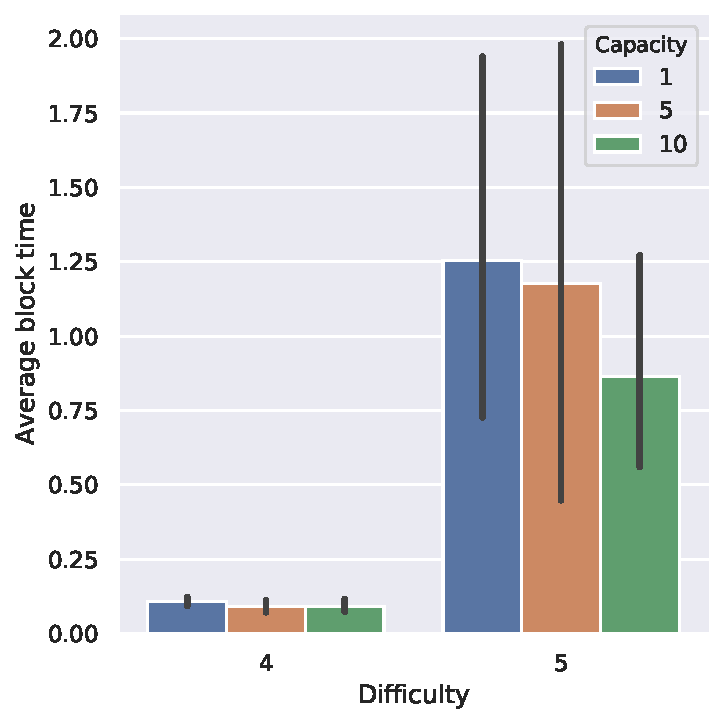
\includegraphics[width=\textwidth]{efficiency_average_block_time.pdf}
        \caption{Μέσο block time}
    \end{subfigure}
    \begin{subfigure}{0.49\textwidth}
        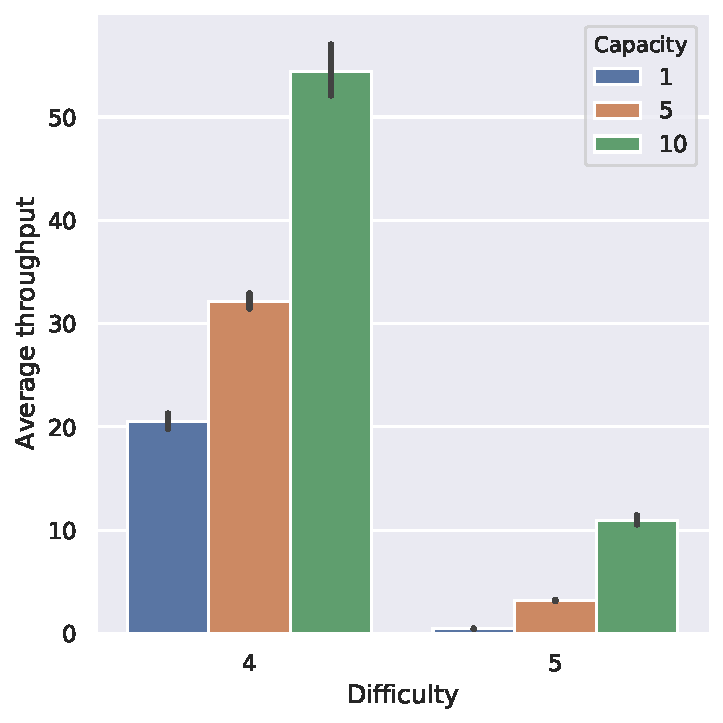
\includegraphics[width=\textwidth]{efficiency_average_throughput.pdf}
        \caption{Μέσο throughput}
    \end{subfigure}
    \caption{Απόδοση}
\end{figure}

\paragraph{Παρατηρήσεις}

Εύκολα βλέπουμε ότι τα αποτελέσματά μας συνάδουν με τα θεωρητικώς αναμενόμενα. Είναι εμφανές ότι η αύξηση του difficulty κατά 1 αυξάνει δραματικά το block time και μειώνει δραματικά το throughput. Όσον αφορά το capacity επιβεβαιώνουμε ότι η αύξηση του capacity αυξάνει σημαντικά το throughput, ενώ παρατηρούμε ότι οδηγεί σε μια σχετική μείωση του block time, ειδικά όταν όταν αυξάνεται από 1 σε 5. Παρόλα αυτά είναι εμφανές ότι δεν υπάρχει κάποια ουσιώσης συχέτιση μεταξύ capacity και block time.

\subsubsection{Κλιμακωσιμότητα}

Σε δεύτερη φάση επαναλαμβάνουμε τις μετρήσεις μας έχοντας σηκώσει αυτή τη φορά 10 servers για τις ίδιες όμως τιμές των παραμέτρων. Ήτοι μελετούμε την κλιμακωσιμότητα του συστήματός μας, όταν διπλασιάζονται οι κόμβοι. Θυμίζουμε πως δεδομένης της ύπαρξης 10 πυρήνων συνολικά δεν αναμένουμε χειροτέρευση της επίδοσης λόγω έλλειψης πόρων στο cluster μας, όπως θα συνέβαινε με περισσότερους από 10 κόμβους. Τα αποτελέσματά μας παρατίθενται στο σχημα 2.

\begin{figure}[!ht]
    \begin{subfigure}{\textwidth}
        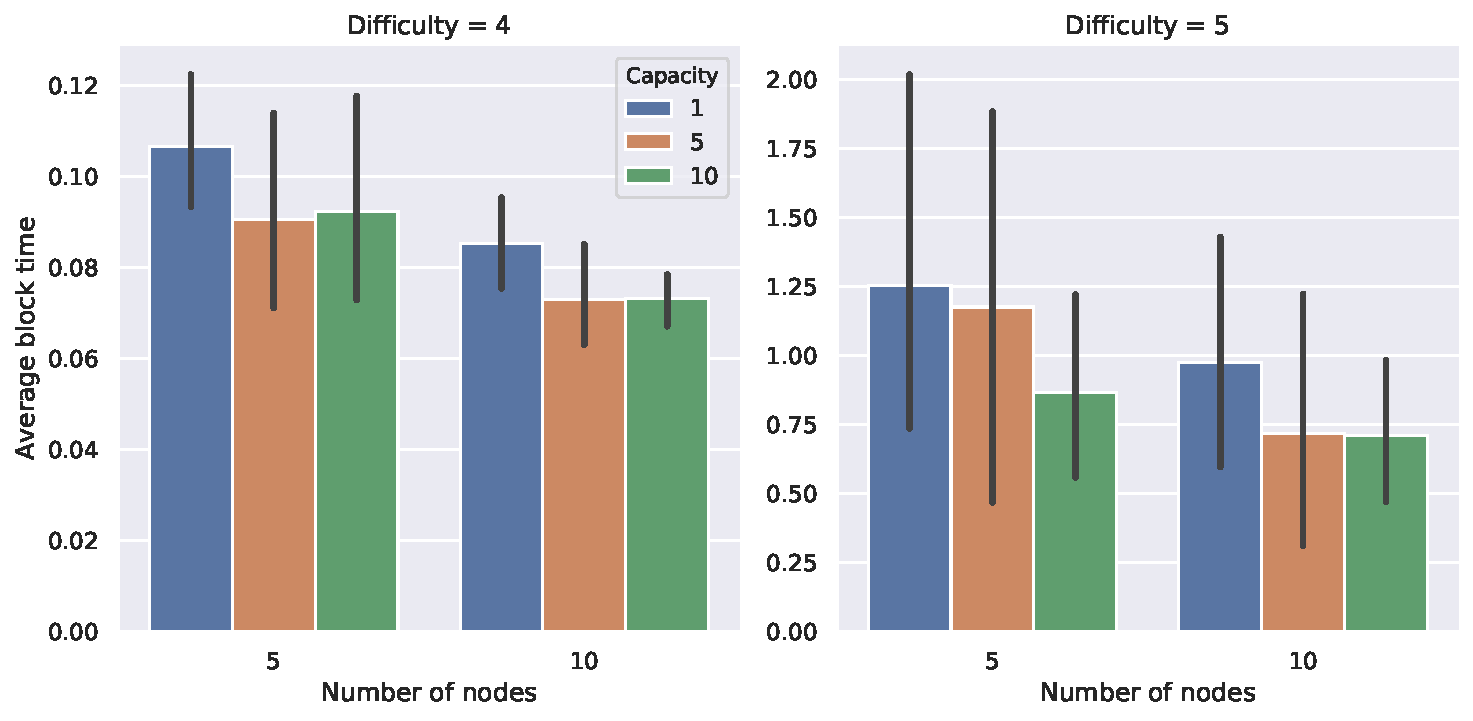
\includegraphics[width=\textwidth]{scalability_average_block_time.pdf}
        \caption{Μέσο block time}
    \end{subfigure}
    \begin{subfigure}{\textwidth}
        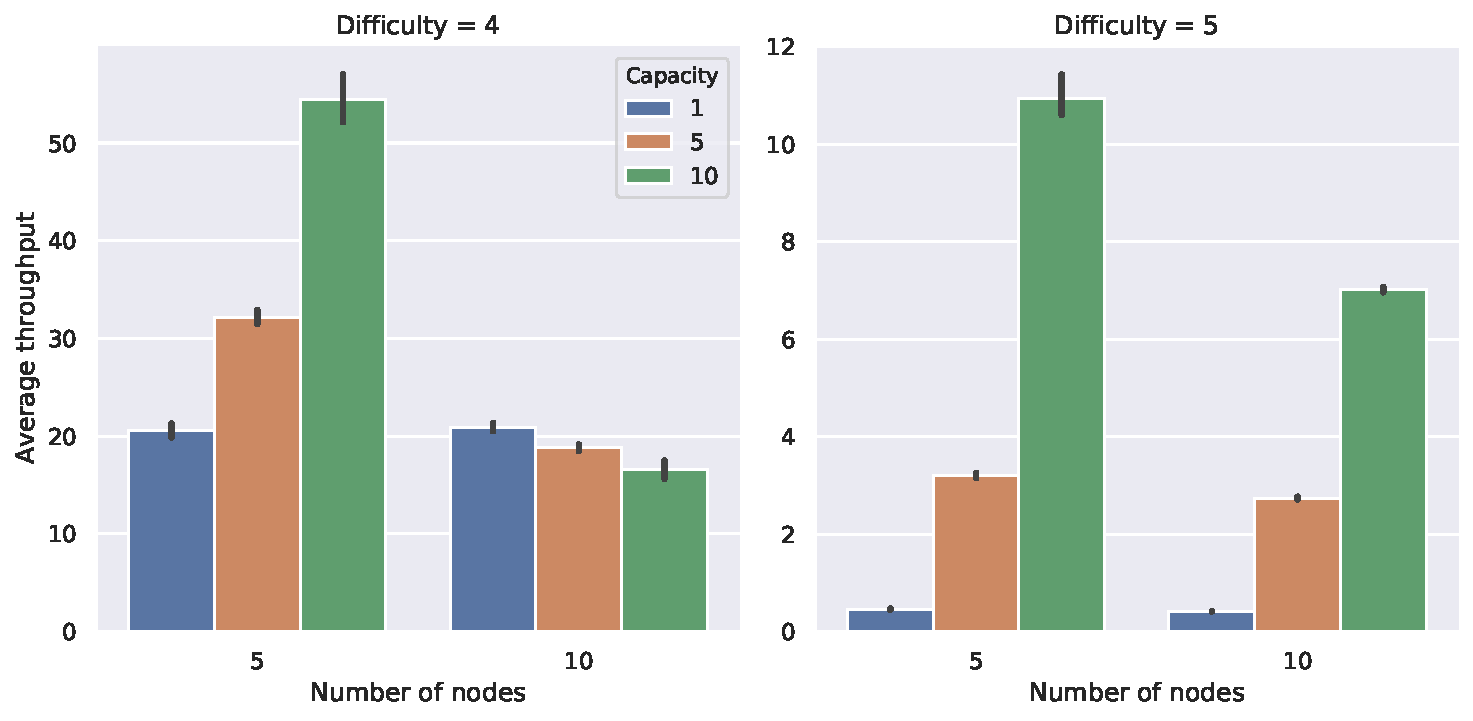
\includegraphics[width=\textwidth]{scalability_average_throughput.pdf}
        \caption{Μέσο throughput}
    \end{subfigure}
    \caption{Κλιμακωσιμότητα}
\end{figure}

\paragraph{Παρατηρήσεις}

Πάλι μπορούμε εύκολα να διακρίνουμε τη συνάφεια των αποτελεσμάτων μας με τις θεωρητικές παρατηρήσεις. Όπως αναμέναμε το block time μειώνεται με την αύξηση των κόμβων, όχι βέβαια γραμμικά, όπως θα συνέβαινε αν οι κόμβοι έκαναν mine τα ίδια blocks συνέχεια, πράγμα που δε συμβαίνει στην πράξη. Αναφορικα με τις παραμέτρους του συστήματος, βλέπουμε πρακτικά την ίδια συμπεριφορά που είδαμε για 5 κόμβους. Εξαίρεση αποτελεί το throughput για 10 κόμβους και difficulty 4, που φαίνεται να μην ευνοείται από την αύξηση του capacity. Όπως βλέπουμε στο σχήμα 3, που αναπαριστά το μέσο πλήθος conflicts που χρειάστηκε να γίνουν resolved, στις προβληματικές παραμέτρους παρατηρείται ένα τεράστιο πλήθος conflicts, λόγω του συνδυασμού πολλών κόμβων με εύκολο mining. Επομένως το throughput δεν μπορεί να βελτιωθεί με το capacity για το συγκεκριμένο συνδυασμό.

\begin{figure}[!ht]
    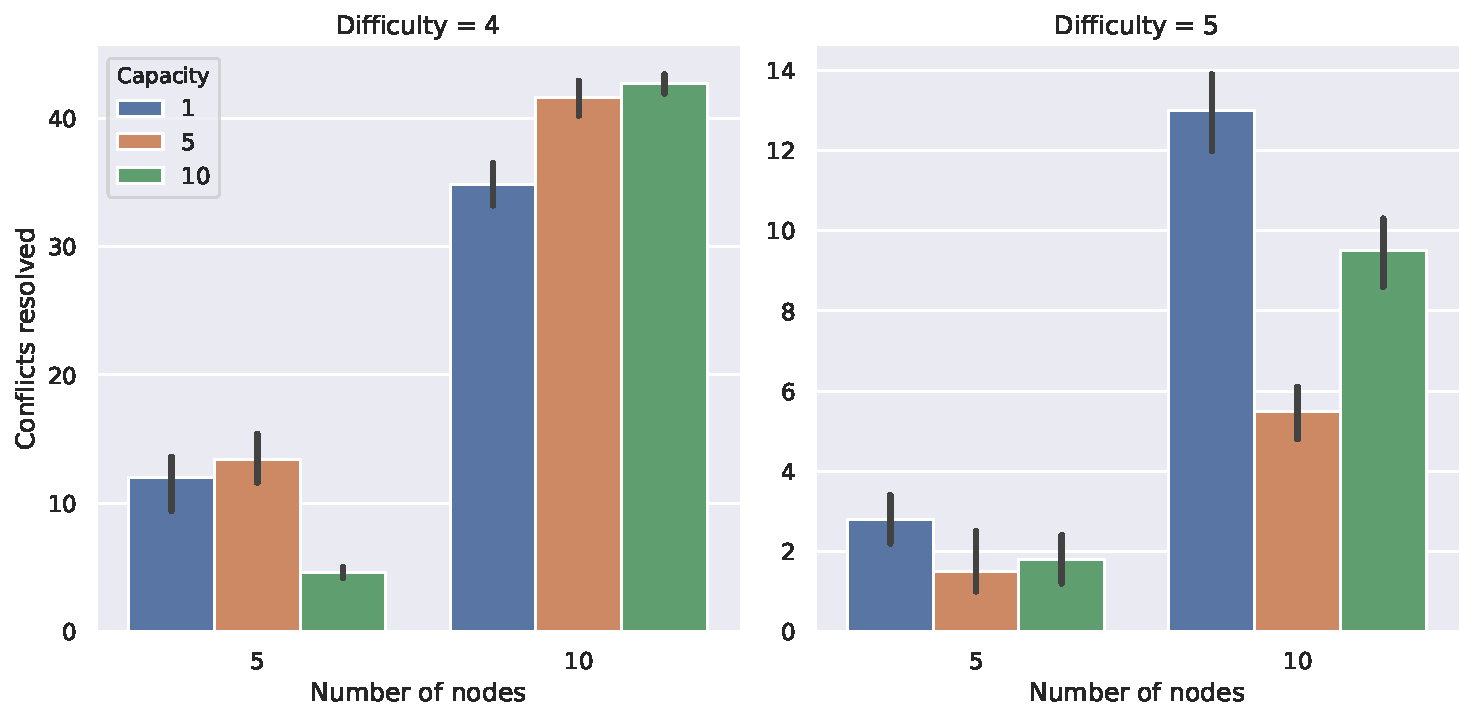
\includegraphics[width=\textwidth]{scalability_conflicts_resolved.pdf}
    \caption{Consensus}
\end{figure}

\paragraph{Η (μη) κλιμακωσιμότητα του throughput} Όσον αφορά το throughput, βλέπουμε ότι είτε μειώνεται με την αύξηση των κόμβων είτε μένει σταθερό. Θυμίζουμε εδώ πως αύξηση των κόμβων εν προκειμένω συνεπάγεται αύξηση της συνολικής υπολογιστικής δύναμης με αντίστοιχη ωστόσο αύξηση των συναλλαγών προς εξυπηρέτηση. Επομένως θέλουμε το σύστημά μας να μπορεί να αντεπεξέλθει με την ίδια ταχύτητα σε περισσότερες αιτήσεις, αν του δώσουμε περισσότερους κόμβους. Πράγματι βλέπουμε ότι στις μισές περιπτώσεις αυτό συμβαίνει. Για μεγάλο capacity όμως και για μεσαίο capacity και μικρο difficulty ωστόσο, είδαμε ότι το σύστημά μας υποφέρει από conflicts. Είναι επομένως αναμενόμενο να περιορίζεται η κλιμάκωση σε εκείνες τις περιπτώσεις.

\end{document}
